\documentclass[11pt, a4paper]{article}

\usepackage{graphicx}
\usepackage[a4paper,top=3cm,bottom=2cm,left=2cm,right=2cm,marginparwidth=1.75cm]{geometry}
\usepackage[english]{babel}
\usepackage[utf8x]{inputenc}
\usepackage{subfig}
\usepackage{float}
\usepackage{amsmath}
\usepackage{amssymb}
\usepackage{mhchem}
\usepackage{hyperref}
\usepackage{tikz}
\usepackage{cancel}

\graphicspath{ {./images} }
\newcommand*{\qed}{\hfill\ensuremath{\quad\square}}%
\newcommand*{\rad}{\ensuremath{\,\text{rad}}}
\newcommand*{\R}{\ensuremath{\mathbb{R}}}
\newcommand*{\C}{\ensuremath{\mathbb{C}}}
\renewcommand*{\Re}{\operatorname{Re}}
\renewcommand*{\Im}{\operatorname{Im}}
\renewcommand*{\epsilon}{\varepsilon}
\renewcommand*{\phi}{\varphi}

\makeatletter
\renewcommand*\env@matrix[1][*\c@MaxMatrixCols c]{%
  \hskip -\arraycolsep
  \let\@ifnextchar\new@ifnextchar
  \array{#1}}
\makeatother

\newtheorem{theorem}{Theorem}

%------------------------------------------------
%Templates for images and figures
% \begin{figure}[h]
%   \centering
%   \subfloat[caption 1]{{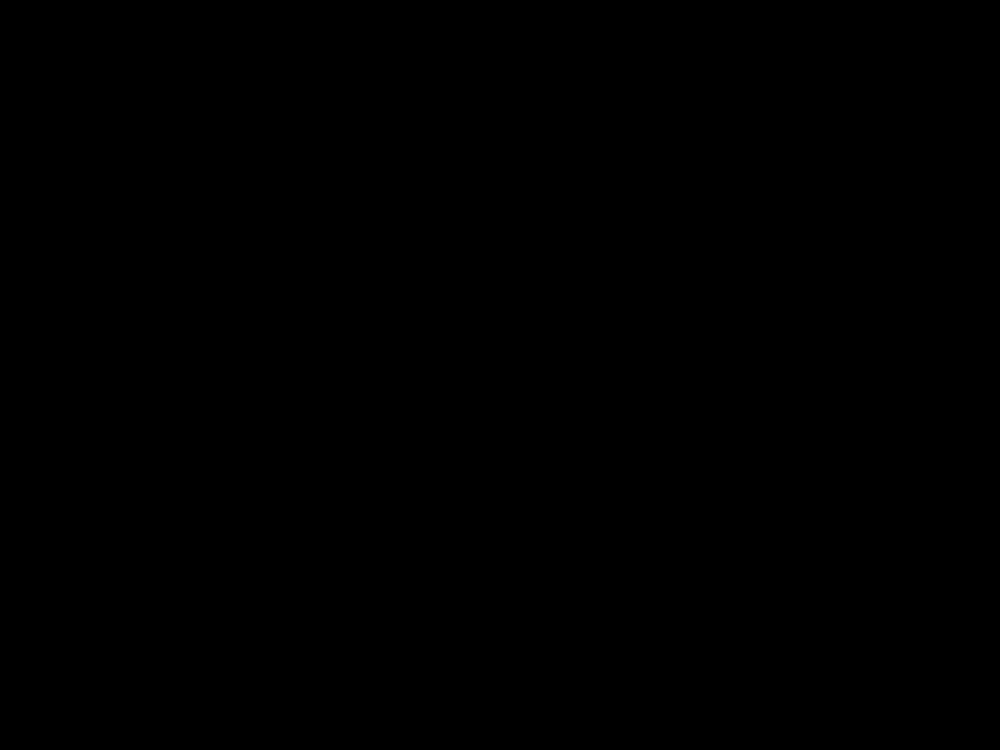
\includegraphics[width=30mm]{images/placeholder.png}}}%
%   \qquad
%   \subfloat[caption 2]{{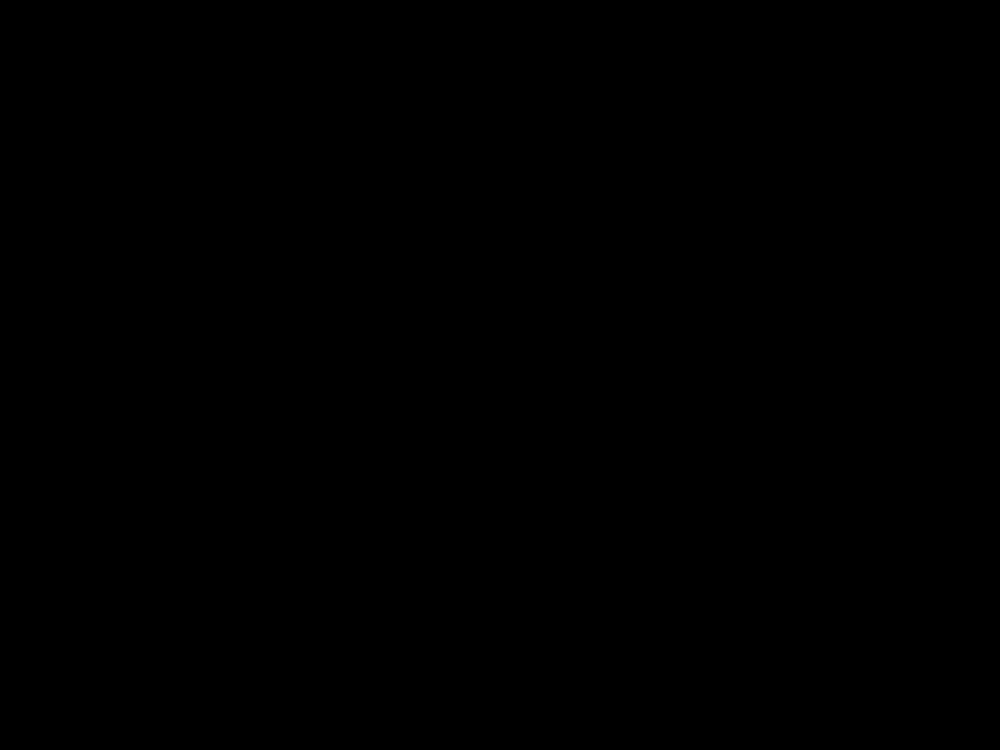
\includegraphics[width=30mm]{images/placeholder.png}}}%
%   \caption{Description}
% \end{figure}

% \begin{figure}[h]
%   \centerline{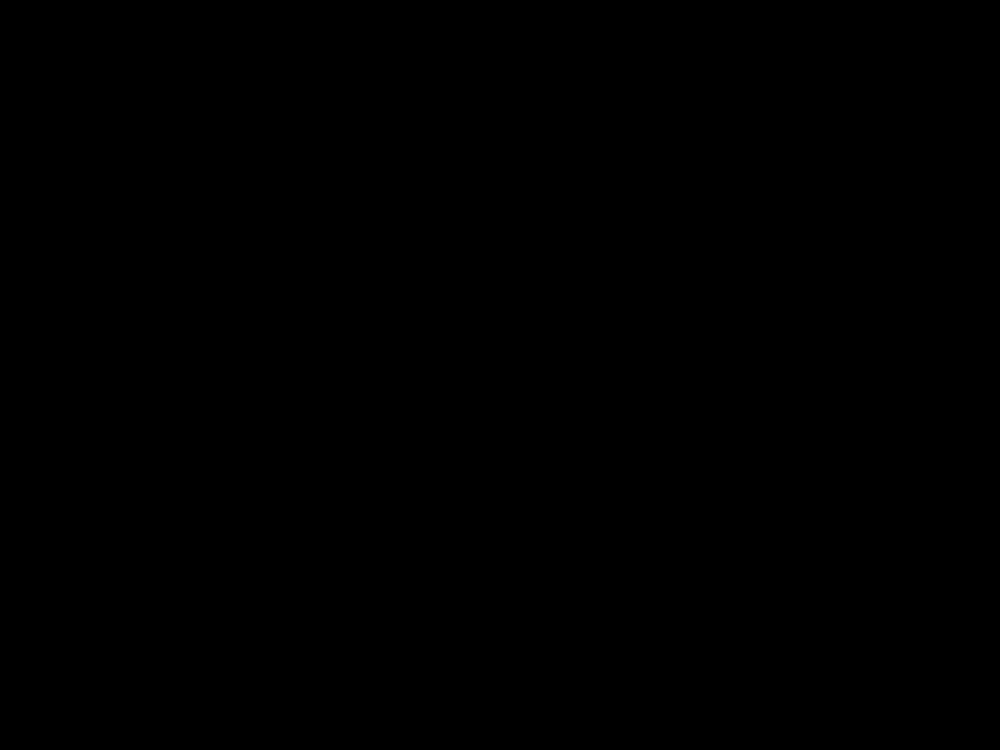
\includegraphics[width=50mm]{images/placeholder.png}}
%   \caption{Description}
% \end{figure}

%Template for a simple table 
%\begin{table}[h]
%   \caption{Description} %title of the table
%   \centering % centering table
%   \begin{tabular}{l rr} % creating three columns
%     \hline\hline %inserting double-line
%     & & \\ [0.5ex] % Insert half line vertical spacing
%     \hline % inserts single-line
%     & & \\ 
%     & & \\
%     & & \\
%     & & \\
%   \hline % inserts single-line
%   \end{tabular}
%   \label{tab:hresult}
% \end{table}
%-----------------------------------------------

\begin{document}
\setcounter{equation}{0}
\setcounter{section}{10}

\section{Thermofluid Lecture 11: Exergy (03/06/2020)}

\subsection{Defining exergy}
Exergy is defined as the maximum amount of work a system can deliver relative to it's surroundings. This happens when a system undergoes a perfectly reversible process from it's initial state to it's dead state. A dead state refers to the final state a system that has reached perfect equilibrium with it's surroundings.


\subsection{Mathematically describing exergy}
We can use the first law to describe the total difference in energy of a system and it's surroundings (The subscript $c$ will be used for the combination $system+enviroment$):
\begin{equation}
  \Delta E_c = \Delta E_{sys} + \Delta E_{env} = Q_c - W_c
\end{equation}
Where $\Delta E_env = \Delta U + \Delta KE + \Delta PE$. Since changing the kinetic and potential energy of the enviroment is very difficult we usually just set these terms to $0$ (with some exceptions a wind turbine for example can cause considerably change in the kinetic energy of surrounding gas). This would leave us with the following:
\begin{align}
  \Delta E_{env} = \Delta U_{env} &= Q_{env} - W_{env}\\
  &= \int_1^2 T\,dS - \int_1^2 p\,dV
\end{align} 
Surroundings of a system are usually pretty big. Because of this saying that pressure and temperature remain more or less constant is a pretty good approximation. The pressure and temperature of a system are usually denoted as $p_0$ and $T_0$. Solving the previous integrals for constant $P$ and $T$ will give the following:
\begin{equation}
  \Delta U_{env} = T_0\Delta S_{env} - p_0 \Delta V_{env}
\end{equation}
Where $\Delta V_{env} = - \Delta V_{sys}$ and $\Delta S_c = \Delta S_{env} + \Delta S_{sys}$. The dead state cannot have any kinetic or potential energy as this would reduce the potential work which can be done. Thus we can state that:
\begin{equation}
  \Delta E_{sys} = U_0 - E_{initial}
\end{equation}
We can then solve for potential work as follows:
\begin{equation}
  W_c = (U - U_0) - p_0(V-V_0) - T_0(S-S_0) + KE + PE - T_0\Delta S_c
\end{equation}
If there is no transfer of energy via heat into or out of the surroundings we get:
\begin{equation}
  \Delta S_c = \left. \cancelto{0}{\int \frac{\delta Q}{T}} \right|_{int\;rev} + \sigma
\end{equation}
Which leaves us with the following expression:
\begin{equation}
  B = W_c = (U - U_0) - p_0(V-V_0) - T_0(S-S_0) + KE + PE - T_0\sigma
\end{equation}
Where $B$ is used to denote the exergy.


\subsection{Exergy analysis of a closed system}
Rather then looking at the value of total exergy we can consider the difference in exergy between 2 different states. This gives us a better way to quantify losses. The difference in exergy between 2 states is given as:
\begin{equation}
  E_2 - E_1 = (U_2 - U_1) - p_0(V_2-V_1) - T_0(S_2-S_1)
\end{equation}
We already know the following:
\begin{gather}
  \Delta U = \int_1^2 \delta Q - W_{12}\\
  \Delta S = \left.\int_1^2 \frac{\delta Q}{T} \right|_b + \sigma \Rightarrow T_0\Delta S = T_0 \left.\int_1^2 \frac{\delta Q}{T} \right|_b + T_0\sigma
\end{gather}
Subtracting these expressions from eachother gives:
\begin{equation}
  \Delta U - T_0\Delta S = \int_1^2 \delta Q - T_0 \left.\int_1^2 \frac{\delta Q}{T} \right|_b -W_{12} - T_0\sigma
\end{equation}
We can then find an expression for exergy by adding back the $p_0(V_2 - V_1)$ term.
\begin{equation}
  B = \int_1^2 \delta Q - T_0 \left.\int_1^2 \frac{\delta Q}{T} \right|_b -W_{12} - T_0\sigma + p_0(V_2 - V_1)
\end{equation}
By doing a bit of algebra we can rewrite this and express exergy for a closed system as:
\begin{equation}
  \Delta B = \left. \int_1^2 \left(1 - \frac{T_0}{T}\right)\delta Q \right|_b - \left[ W - p_0(V_2 - V_1)\right] - T_0\sigma
\end{equation}
From this expression we can conclude that exergy can be changed by either energy transfer via heat or work. Aditionally the $-T_0\sigma$ term also implies that some exergy is destroyed due to increase in entropy. We can take the time derrivative of the previous expression to get the exergy balance for systems with time dependence:
\begin{equation}
  \frac{dB}{dt} = \left. \int_1^2 \left(1 - \frac{T_0}{T}\right)\delta\dot{Q} \right|_b - \left[ \dot{W} - p_0\frac{dV}{dt}\right] - T_0\dot{\sigma}
\end{equation}


\subsection{Exergetic efficiency}
Exergetic efficiency, sometimes also called second law efficiency, is the efficiency relative to the maximum possible efficiency. This is different from the earlier definition of thermal efficiency:
\begin{equation}
  \eta_{th} \equiv \frac{\text{benefit}}{\text{cost}}
\end{equation}
Second law efficiency can be found by using the exergy equations we found earlier. This will give:
\begin{equation}
  \eta_{II} = \frac{\text{exergy recovered}}{\text{exergy expended}} = 1 - \frac{\text{exergy destroyed}}{\text{exergy expended}}
\end{equation}
or in symbolic form:
\begin{equation}
  \eta_{II} = \frac{B_{out}}{B_{in}} = 1 - \frac{(B_{lost} + B_{destroyed})}{B_{in}}
\end{equation}



\end{document}
